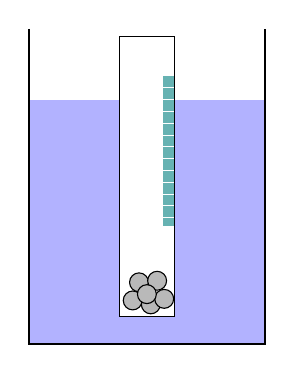
\begin{tikzpicture}
  % water
  \fill[blue!30] (0,0) rectangle (3,3.1);
  % beaker walls (open top)
  \draw[thick] (0,4) -- (0,0) -- (3,0) -- (3,4);
  % inner tube
  \fill[white] (1.15,0.35) rectangle (1.85,3.9);
  \draw (1.15,0.35) rectangle (1.85,3.9);
  % graduated scale
  \fill[teal!60] (1.7,1.5) rectangle (1.85,3.4);
  \foreach \y in {1.6,1.75,...,3.35} { \draw[white] (1.7,\y) -- (1.85,\y); }
  % balls at bottom of tube
  \foreach \c in {(1.32,0.55),(1.55,0.5),(1.72,0.57),(1.4,0.78),(1.63,0.8),(1.5,0.63)} {
    \fill[gray!55] \c circle (0.12);
    \draw \c circle (0.12);
  }
\end{tikzpicture}
